\section{Homework 5}
\subsection{Exercise 4.15}

Relaxation of a boolean LP

A boolean linear program is defined as 
\begin{align}
  \text{minimize} & \quad c^T x \\
  \text{subject to} & \quad Ax \preceq b \\
  & \quad x_i \in \{ 0,1\}, i = 1, \dots, n 
\end{align}
This linear program can be relaxed by replacing the integer constraint with linear inequalities
\begin{align}
  \text{minimize} & \quad c^T x \\
  \text{subject to} & \quad Ax \preceq b \\
  & \quad 0 \leq x_i \leq 1, i = 1,\dots,n
\end{align} 
\subsubsection{Part a}
The optimal value of the LP relaxation is a lower bound on the optimal value. We can use a geometric example to prove this. Since the affine constraints in both the relaxed and original LP form a polyhedron. There are distinct vertex that either do or don't coincide with an integer point. In the event that the polyhedron's vertices land on the integer point, then if the optimal value lies on that vertex, then the optimal value for both the relaxed problem and original problem are equal. In the event that the vertex does not lie on the integer point, then the solution to the relaxed LP is a lower bound on the optimal value of the boolean LP.  \\ \\
The image below illustrates how the vertices lie on integers and therefore the optimal values would be equal. However, if the polyhedron extended out a bit to $(0,0.5),(0.5,0)$ as opposed to $(0,1),(1,0)$ then the relaxed polyhedron would be a strict lower bound.
\begin{figure}[htbp]
  \centerline{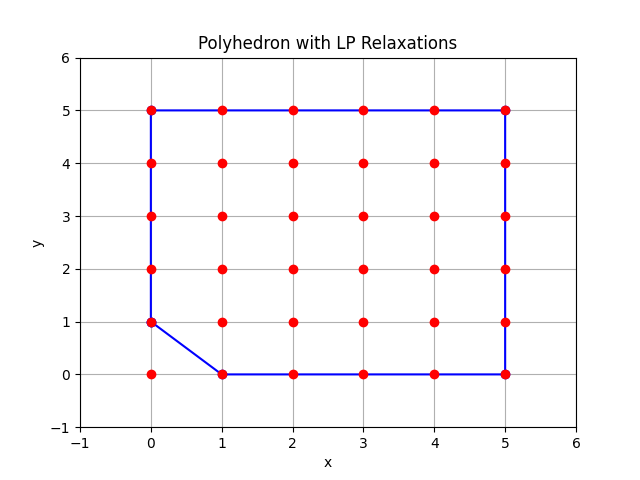
\includegraphics[width=0.50\textwidth]{hw5/lp_relaxed_polyhedron.png}}
  \caption{A polyhedron in $\mathbb{R}^2$ with points at each integer}
  \label{fig:lp_relaxed_polyhedron}
\end{figure} 
\subsubsection{Part b}
This section was also answered in part a. However, the solutions for the relaxation and original problem will coincide whenever the polyhedron created by the given $A$ and $b$ lie on an integer.

\subsection{Exercise 4.60}
\begin{itemize}
  \item $x$: An allocation strategy that dictates the portion of the wealth allocated to each $i$ asset. $x \in \mathbb{R}^n$
  \item $n$: Number of assets
  \item $N$: Number of periods
  \item $W(t-1)$: Amount of wealth at the beginning of period $t$ or end of period $t-1$
  \item $\lambda(t)$: Total return during period $t$. $\lambda(t) = \frac{W(t)}{W(t-1)}$. A random variable with $m$ possible values.
  \item $\frac{1}{N} \sum_{t=1}^{N} \log \lambda(t)$: Growth rate of the investment over $N$ periods.
  \item $m$: Number of deterministic return scenarios.
  \item $\pi_j$: Probability of getting scenario $j$ at any given period. $\pi_j = \textbf{prob}(\lambda(t) = p_j^T x)$
  \item $p_{ij}$: The return for asset $i$ over one period in which scenario $j$ occurs.
\end{itemize}

Our goal here is to maximize our total expected long-term growth rate. First, for my understanding, I am going to derive the formula for the growth rate.
\begin{equation}
  \begin{aligned}
    W(N) = W(0) \prod_{t=1}^{N} \lambda(t) \\
    \frac{1}{N} \log (W(N) - W(0)) = \frac{1}{N} \log \prod_{t=1}^{N} \lambda(t) \\
    = \frac{1}{N} \sum_{t=1}^N \log \lambda(t)
  \end{aligned}
\end{equation}
Now, with this I am going to derive the formula for long term growth rate.

\begin{equation}
  \begin{aligned}
    \lim_{N \to \infty} \frac{1}{N} \sum_{t=1}^N \log \lambda(t) = \mathbb{E}[\log \lambda(t)] \\ 
    = \sum_{j=1}^m \pi_j \log p_j^\top x
  \end{aligned}
\end{equation}

The final optimization problem is:

\begin{align}
  \text{maximize} & \quad \sum_{j=1}^m \pi_j \log p_j^\top x \\
  \text{subject to} & \quad x \succeq 0  \\
  & \quad \textbf{1}^\top x = 1
\end{align}

This question requires that we prove that the above optimization problem is a convex optimization problem. For convention, the problem is turned into

\begin{align}
  \text{minimize} & \quad -\sum_{j=1}^m \pi_j \log p_j^\top x \\
  \text{subject to} & \quad x \succeq 0  \\
  & \quad \textbf{1}^\top x = 1
\end{align}

For this to be a convex problem, the objective function and inequalities must be convex, and the equality constraints must be affine.

Firstly, the objective function is convex:
\begin{itemize}
  \item $p_j^\top x $ is an affine function of the variable $x$
  \item $ \pi_j \log u \text{ with } u = (p_j^\top x)$ is a concave function of the variable $u$, which itself is an affine function of $x$. The function is then multiplied by a non-negative weight which maintains its concavity
  \item $\sum v \text{ with } v = \pi_j \log p_j^\top x$ is a sum of concave functions which is concave.
  \item $- w \text{ with } w = \sum_{j=1}^m \pi_j \log p_j^\top x$ is the negative of a concave function which is convex.
\end{itemize}

Clearly, the inequality is convex as it is the cone $\mathbb{R}^m_{+}$

The equality is indeed affine, therefore the optimization problem is convex!

\subsection{Exercise 5.13}
\subsubsection{Part a}
This part involves finding the lagrange dual of the boolean LP, which we can use to get a lower bound on the original optimization problem.

\begin{align}
  \text{minimize} & \quad c^T x \\
  \text{subject to} & \quad Ax \preceq b \\
  & \quad x_i(1-x_i) = 0
\end{align}

\begin{equation}
  \begin{aligned}
    L(x, \lambda, \nu) = c^T x + \lambda^T(Ax - b) + \nu^T (x- \textbf{diag}(x)x) \\  
    = c^T x + \lambda^TAx - \lambda^T b + \nu^T x- x^T \textbf{diag}(\nu) x
  \end{aligned}
\end{equation}

\begin{equation}
  \begin{aligned}
    \nabla L(x, \lambda, \nu) = c + A^T \lambda + \nu - 2 \textbf{diag}(\nu) x \\
    2 \textbf{diag}(\nu) x = c + A^T \lambda + \nu \\
    x = \frac{1}{2} \textbf{diag}(\nu) ^{-1} (c + A^T \lambda + \nu )\\
  \end{aligned}
\end{equation}

\begin{equation}
  \begin{aligned}
    g(\lambda, \nu) = -\lambda^T b + (c + A^T \lambda + \nu )^T x - \frac{1}{2} x^T(c + A^T \lambda + \nu) \\ 
    = -\lambda^T b + \frac{1}{2} (c + A^T \lambda + \nu)^T \frac{1}{2} \textbf{diag}(\nu) ^{-1} (c + A^T \lambda + \nu ) \\ 
    = -\lambda^T b + \frac{1}{4} (c + A^T \lambda + \nu)^T (\textbf{diag}(\nu) ^{-1} (c + A^T \lambda + \nu ))
  \end{aligned}
\end{equation}

\begin{equation}
  g(\lambda, \nu) = 
  \begin{cases}
    -\lambda^T b + \frac{1}{4} z^T \tilde{D} z & \nu \succeq 0 \\
    -\infty & o/w
  \end{cases}
\end{equation}
where $z = (c + A^T \lambda + \nu) \text{ and } \tilde{D} = \textbf{diag}(\nu) ^{-1}$

Solving for the maximum here we have the optimization problem

\begin{align}
  \text{maximize} & \quad g(\lambda, \nu) = -\lambda^T b - \frac{1}{4} (c + A^T \lambda + \nu)^T (\textbf{diag}(\nu) ^{-1} (c + A^T \lambda + \nu ))  \\
  \text{subject to} & \quad \lambda \succeq 0 \\
  & \quad \nu \succeq 0 
\end{align}

\subsubsection{Part b}
Now, first we derive the lagrangian dual of the LP relaxation 
\begin{align}
  \text{minimize} & \quad c^T x \\
  \text{subject to} & \quad Ax \preceq b \\
  & \quad \textbf{0} \preceq x \preceq \textbf{1}
\end{align}

\begin{equation}
  \begin{aligned}
    L(x, \lambda, \nu_1, \nu_2) = c^T x + \lambda^T (Ax-b) - \nu_1^T (x) + \nu_2^T (x-1) \\
    = (c+ A^T \lambda -\nu_1 + \nu_2 )^T x - \lambda^T b - \textbf{1}^T \nu_2
  \end{aligned}
\end{equation}

\begin{equation}
  \begin{aligned}
    \nabla L(x, \lambda, \nu_1, \nu_2) = c + A^T \lambda - \nu_1 + \nu_2 \\
    0 =  c + A^T \lambda - \nu_1 + \nu_2
  \end{aligned}
\end{equation}

\begin{equation}
  g(\lambda, \nu_1, \nu_2) = 
  \begin{cases}
    -\lambda^T b - \textbf{1}^T \nu_2 & 0 =  c + A^T \lambda - \nu_1 + \nu_2 \\
    -\infty & o.w.
  \end{cases}
\end{equation}

The optimization problem with this lagrangian is 

\begin{align}
  \text{maximize} & \quad   g(\lambda, \nu_1, \nu_2) = -\lambda^T b - \textbf{1}^T \nu_2  \\
  \text{subject to} & \quad  0 =  c + A^T \lambda - \nu_1 + \nu_2 \\
  & \lambda \succeq 0, \nu_1 \succeq 0, \nu_2 \succeq 0 \quad 
\end{align}

That is apparently the same as the above but I can't quite understand why

\subsection{Exercise 6.2}
This exercise involves finding the solution of the scalar norm approximation problem with $l_1, l_2, l_\infty$
\begin{align}
  \text{minimize} & \quad \| x \textbf{1} - b \|
\end{align}
Where $x \in \mathbb{R}$ and $b \in \mathbb{R}^n$

\subsubsection{Part a}
$l_2$ norm
\begin{align}
  \text{minimize} & \quad \| x \textbf{1} - b \|_2
\end{align}


\begin{equation}
  \begin{aligned}
    f(x) = \frac{1}{n} \sum_{i=1}^n (x-b_i)^2 \\
    \nabla f(x) = \frac{2}{n}\sum_{i=1}^n (x-b_i) \\
    \sum_{i=1}^n b_i = nx \\ 
    x = \frac{1}{n} \sum_{i=1}^n b_i \text{ or } \frac{\textbf{1}^T b}{n}
  \end{aligned}
\end{equation}

\subsubsection{Part b}
$l_1$ norm
\begin{align}
  \text{minimize} & \quad \| x \textbf{1} - b \|_1
\end{align}


\begin{equation}
  \begin{aligned}
    f(x) = \frac{1}{n} \sum_{i=1}^n |x-b_i|
  \end{aligned}
\end{equation}
The answer to this is the median of the vector $b$.

\subsubsection{Part c}
$l_1$ norm
\begin{align}
  \text{minimize} & \quad \| x \textbf{1} - b \|_\infty
\end{align}
Here we are minimizing the maximum absolute distance between any of the components of $b$ and $x$
\begin{equation}
  \begin{aligned}
    \max_i \{ |x-b_i| \}
  \end{aligned}
\end{equation}
The only two important numbers in $b$ are $b_{min}, b_{max}$. In order to minimize the distance between $x$ and these two points, $x$ is set to the midrange between those two points

\begin{equation}
  x = \frac{b_{min} + b_{max}}{2}
\end{equation}

\subsection{Additional Problem HW5.2}
Formulating different optimization problems as semidefinite programs with the variable $x \in \mathbb{R}^n$ and
\begin{equation}
  F(x) = F_0 + x_1F_1 + x_2F_2 + \dots x_n F_n
\end{equation}
where $F_i \in \mathbb{S}^m$.

A semidefinite program is an optimization problem in the form 
\begin{align}
  \text{minimize} & \quad c^T x \\
  \text{subject to} & \quad x_1 F_1 + x_2F_2 + \dots x_nF_n + G \preceq 0 \\
  & \quad Ax = b
\end{align}
where $F_i, G \in \mathbb{S}^k$
\subsubsection{Part a}
Minimize $f(x) = c^T F(x)^{-1} c \text{ where } c \in \mathbb{R}^m$:
\begin{align}
  \text{minimize} & \quad y \\
  \text{subject to} & \quad y \geq c^T F(x)^{-1} c
\end{align}

\begin{equation}
  \begin{aligned}
    y \geq c^T F(x)^{-1} c \\
    y F(x) \succeq c c ^T \\
    y F(x) - cc^t \succeq 0
  \end{aligned}
\end{equation}

\begin{align}
  \begin{bmatrix}
     F(x) & c \\
     c^T & y
  \end{bmatrix}
  \succeq 0 
\end{align}

\subsubsection{Part b}
Minimize $f(x) = \max_{i} c_i^T F(x)^{-1} c_i$ 

\begin{align}
  \text{minimize} & \quad y \\
  \text{subject to} & \quad y \geq c_i^T F(x)^{-1} c_i \forall i \in \{ 1, \dots, K \}
\end{align}

\begin{align}
  \begin{bmatrix}
     F(x) & c_i \\
     c_i^T & y
  \end{bmatrix}
  \succeq 0 & \forall i
\end{align}

\subsubsection{Part c}
Minimize $f(x) = \sup_{\| c \|_2 \leq 1} c^T F(x)^{-1} c$

\begin{align}
  \text{minimize} & \quad \text{maximize } y\\
  \text{subject to} & \quad y \geq c^T F(x)^{-1} c  \\
  & \quad \| c \|_2 \leq 1
\end{align}
Don't really get this one but the answer is

\begin{align}
  \begin{bmatrix}
     F(x) & I \\
     I & yI
  \end{bmatrix}
  \succeq 0 
\end{align}

\subsection{Additional Problem HW5.5}
Maximizing house profit in a gamble and imputed probabilities.
\begin{itemize}
  \item $n$: number of participants
  \item $m$: number of outcomes that the participants can bet on
  \item $q_i$: number of gambling contracts that a participant can bet on $q_i > 0$
  \item $p_i$: price of gambling contract $i$
  \item $\mathbb{S}_i$: $\mathbb{S}_i \subset \{ 1,\dots, m \}$ A set the participant $i$ specifies that they are betting the outcome will lie in. 
  \item $x_i$: The number of contracts that the house sells to the participant. If the true outcome $j$ is in $\mathbb{S}_i$, the partipant will receive \$1 per $x_i$ the house has sold them. $0 \leq x_i \leq q_i$
  \item $R(x)$: Revenue that the house collects. $R(x) = p^T x$ or $R(x) = p_1x_1 + \dots + p_nx_n$
  \item $C(x)$: Cost that the house has to pay out to the participants that depends on outcome j. $C(x) = \sum_{j \in \mathbb{S}_i} x_i$ which is a random variable that depends on the outcome.
  \item $P(x)$: House profit. $R(x) - C(x)$
\end{itemize}

\subsubsection{Part a}
This section involves finding the optimal worst-case house strategy.

Worst case profit is defined as below

\begin{equation}
  P_{wc}(x) = p^T x - \max_{j} \sum_{j \in \mathbb{S}_i } x_i
\end{equation}
The house wants to solve the following optimization problem.

\begin{align}
  \text{maximize} & \quad  p^T x - \max_{j} \sum_{j \in \mathbb{S}_i } x_i \\
  \text{subject to} & \quad 0 \preceq x \preceq q
\end{align}

We can create a series of vectors $z_i \in \mathbb{R}^m$ where each entry is 1 if the outcome $j$ is in the set $\mathbb{S}_i$ and it is 0 otherwise. The multiplication of the two would correspond to a vector with each outcome stored in a vector. $z* = \max_{j} \{ x_i z_i \} \forall i$. This represents the maximum loss on each participant. The optimization problem is then turned into

\begin{align}
  \text{minimize} & \quad p^T x - \textbf{1}^T z^* \\
  \text{subject to} & \quad 0 \preceq x \preceq q \\
  & \quad z_i^* \geq \max_j \{ x_i \textbf{z}_i \} \forall i
\end{align}
With crazy confusing notation.

\subsubsection{Part b}
I am going to borrow a little from the solutions notation to turn mine into an LP.

We can turn the answer from part a into an LP by collecting the previous vector into a matrix $Z$ and introducing a new scalar variable.

\begin{align}
  \text{minimize} & \quad p^T x - z \\
  \text{subject to} & \quad z \textbf{1} \succeq Zx \\
  & \quad 0 \preceq x \preceq q
\end{align}

We can now find the dual from this LP

\begin{equation}
  \begin{aligned}
    L(x,z, \lambda_1, \lambda_2, \lambda_3) = p^T x - z + \lambda_1^T(Zx - z\textbf{1}) - \lambda_2^T(x) + \lambda_3^T(x-q) \\ 
    = (p+ Z^T \lambda_1 - \lambda_2 + \lambda_3 )^T x - z + z\lambda_1^T \textbf{1} - \lambda_3^T q
  \end{aligned}
\end{equation}

\begin{equation}
  \begin{aligned}
    \nabla_x L(x,z, \lambda_1, \lambda_2, \lambda_3) = p+ Z^T \lambda_1 - \lambda_2 + \lambda_3 \\
    0 = p+ Z^T \lambda_1 - \lambda_2 + \lambda_3 \\
    \nabla_z L(x,z, \lambda_1, \lambda_2, \lambda_3) = -1 + \lambda_1^T \textbf{1} \\
    1 = \lambda_1^T \textbf{1}
  \end{aligned}
\end{equation}

\begin{equation}
  g( \lambda_1, \lambda_2, \lambda_3) = 
  \begin{cases}
    - \lambda_3^T q & 1 = \lambda_1^T \textbf{1},  0 = p+ Z^T \lambda_1 - \lambda_2 + \lambda_3 \\
    0 & o.w.
  \end{cases}
\end{equation}

The dual optimization problem is as follows

\begin{align}
  \text{maximize} & \quad -\lambda_3^T q \\
  \text{subject to} & \quad 0 = p+ Z^T \lambda_1 - \lambda_2 + \lambda_3 \\
  & \quad 1 = \lambda_1^T \textbf{1} \\
  & \quad \lambda_1 \succeq 0, \lambda_2\succeq 0, \lambda_3 \succeq 0
\end{align}

$\lambda_1 \in \mathbb{R}^n$ is a probability distribution as it sums up to 1 and each value is non-negative. Therefore, we set $\pi = \lambda_1^*$ to get the probability distribution that maximizes both expected and worst case scenario.
